\documentclass[a4paper,11pt,twoside]{article}
%\documentclass[a4paper,11pt,twoside,se]{article}

\usepackage{UmUStudentReport}
\usepackage{verbatim}   % Multi-line comments using \begin{comment}
\usepackage{courier}    % Nicer fonts are used. (not necessary)
\usepackage{pslatex}    % Also nicer fonts. (not necessary)
\usepackage[pdftex]{graphicx}   % allows including pdf figures
\usepackage{listings}
\usepackage{pgf-umlcd}
\usepackage{blindtext}
\usepackage{enumitem}
\usepackage{amsfonts}
\usepackage{mathtools}
%\usepackage{lmodern}   % Optional fonts. (not necessary)
%\usepackage{tabularx}
%\usepackage{microtype} % Provides some typographic improvements over default settings
%\usepackage{placeins}  % For aligning images with \FloatBarrier
%\usepackage{booktabs}  % For nice-looking tables
%\usepackage{titlesec}  % More granular control of sections.

% DOCUMENT INFO
% =============
\department{Department of Computing Science}
\coursename{Parallel Programming 7.5 p}
\coursecode{5DV152}
\title{Exercises, Chapter/Topic 3}
\author{Lorenz Gerber ({\tt{dv15lgr@cs.umu.se}} {\tt{lozger03@student.umu.se}})}
\date{2017-02-16}
%\revisiondate{2016-01-18}
\instructor{Lars Karlsson / Mikael Ränner}


% DOCUMENT SETTINGS
% =================
\bibliographystyle{plain}
%\bibliographystyle{ieee}
\pagestyle{fancy}
\raggedbottom
\setcounter{secnumdepth}{2}
\setcounter{tocdepth}{2}
%\graphicspath{{images/}}   %Path for images

\usepackage{float}
\floatstyle{ruled}
\newfloat{listing}{thp}{lop}
\floatname{listing}{Listing}



% DEFINES
% =======
%\newcommand{\mycommand}{<latex code>}
\DeclarePairedDelimiter{\ceil}{\lceil}{\rceil}
\DeclarePairedDelimiter{\floor}{\lfloor}{\rfloor}

% DOCUMENT
% ========
\begin{document}
\lstset{language=C}
\maketitle
\thispagestyle{empty}
\newpage
\tableofcontents
\thispagestyle{empty}
\newpage

\clearpage
\pagenumbering{arabic}

\section{Introduction}
This report is part of the mandatory coursework. It describes the solutions for several chosen exercises from the course book \cite{pacheco2011}.

\section{3.2 - Generalization of algorithm for trapezoidal rule}
Two functions to adapt the \textit{trapezoidal rule} for \verb+calc\_local\_a+ and \verb+calc\_local\_b+ were written and tested with the source code from the book (\textit{mpi\_trap.c}).

\begin{verbatim}
double calc_local_a(int my_rank, double a, double b, int n, int comm_sz){
  double local_a = 0;
  double h = 0;
  int local_n = 0;
  int rest_n  = 0;

  h = (b-a)/n;
  local_n = n/comm_sz;

  rest_n = n%comm_sz;

  if(my_rank < rest_n){
    local_a = a + my_rank*local_n*h + my_rank*h;
  } else {
    local_a = a + my_rank*local_n*h + rest_n*h;
    local_a += (my_rank-rest_n) * h;
  }

  return local_a;

}


double calc_local_b(int my_rank, double a, double b, int n, int comm_sz){
  double h;
  int local_n;

  h = (b-a)/n;
  local_n = n/comm_sz;

  if (my_rank == (comm_sz-1)){
    return a + my_rank+1*local_n*h;
  } else {
    return calc_local_a(my_rank+1, a, b, n, comm_sz);
  }
}

\end{verbatim}

\section{3.6 - Array distributions}

\subsection*{Block distribution}
Block distribution can be obtained by $b = \floor*{i \div p}$ where $b$ is the block number, $i$ the index of $n$ and $p$ is the number of processes. This solution is however not fair. An improved, fair expression can be devised using a ternary operator:
\begin{equation*}
i< n\bmod p \times \ceil*{n \div p} ? \floor*{i \div \ceil*{n \div p}} : n\mod p + \floor*{(i -n\mod p \times \ceil*{n \div p}) \div \floor*{n\mod p}}
\end{equation*} 

\subsection*{Cyclic distribution}
Cyclic distribution is described by $b = i\mod p$ with $b$ as block number $i$ as index of $n$ and $p$ as number of processes. 

\subsection*{Block cyclic distribution}
Block cyclic distribution can be expressed as $b = \floor*{i \div l} mod p$ where $b$ is block index, $i$ index of $n$, $l$ block length and $p$ number of processes.

\section{3.8 - Tree-structured algorithms for scatter and gather}
\begin{figure}

  \centering
  
\includegraphics[width=1\textwidth]{scatter.png}
  \caption{\textit{This graph shows a tree based implementation of scatter for comm\_sz = 8 and n = 16.}}
  \label{fig:scatter}
\end{figure}
\begin{figure}

  \centering
  
\includegraphics[width=1\textwidth]{gather.png}
  \caption{\textit{This graph shows a tree based implementation of gather for comm\_sz = 8 and n = 16.}}
  \label{fig:gather}
\end{figure}

\section{3.9 - Vector scaling and dot product}
\begin{verbatim}
#include <stdio.h>
#include <mpi.h>
#include <string.h>
#include <stdlib.h>
#include <time.h>


int main(int argc, char *argv[]) {
  int my_rank, comm_sz;
  int n, local_n, local_dotp_sum = 0, scalar, result_dot;
  int* local_vec1;
  int* local_vec2;
  int* vector1;
  int* vector2;

  /* Initializing */
  MPI_Init(NULL, NULL);
  MPI_Comm_rank(MPI_COMM_WORLD, &my_rank);
  MPI_Comm_size(MPI_COMM_WORLD, &comm_sz);
  srand(time(NULL));

  /* Obtaining Data */
  if(my_rank==0 && argc > 1){

    if(strcmp(argv[1], "r") == 0){
      printf("using random data, vector length = %d\n", 100*comm_sz);
      n = 100*comm_sz;
      vector1 = (int *) malloc(100*comm_sz * sizeof(int));
      vector2 = (int *) malloc(100*comm_sz * sizeof(int));

      for(int i = 0; i < n;i++){
	vector1[i] = rand() % 1000;
	vector2[i] = rand() % 1000;
      }
      scalar = rand() % 1000;
    }
    
  } else if (my_rank==0){
     
    printf("enter vector length\n");
    scanf("%d", &n);
    printf("enter integer vector 1\n");

    vector1 = (int *) malloc(n * sizeof(int));
    vector2 = (int *) malloc(n * sizeof(int));

    for(int i = 0; i < n; i++){
      scanf("%d", &vector1[i]);
    }

    printf("enter integer vector 2\n");

    for(int i = 0; i < n; i++){
      scanf("%d", &vector2[i]);
    }

    printf("enter integer scalar\n");
    scanf("%d", &scalar);
  }

  /* Distribute Data */
  MPI_Bcast(&n, 1, MPI_INT, 0, MPI_COMM_WORLD);
  
  local_n = n/comm_sz;
  local_vec1 = (int*) malloc(local_n * sizeof(int));
  local_vec2 = (int*) malloc(local_n * sizeof(int));
  
  MPI_Bcast(&scalar, 1, MPI_INT, 0, MPI_COMM_WORLD);
  MPI_Scatter(vector1, local_n, MPI_INT, local_vec1, local_n, MPI_INT, 0, MPI_COMM_WORLD);
  MPI_Scatter(vector2, local_n, MPI_INT, local_vec2, local_n, MPI_INT, 0, MPI_COMM_WORLD);
 
  /* Calculations */
  /* Calculate Dot Product */
  for(int i = 0;  i< local_n; i++){
    local_vec2[i]*=local_vec1[i];
  }

  /* Calculate vector-scalar product */
  for(int i = 0; i< local_n; i++){
    local_vec1[i]*=scalar;
  }

  /* Summing for dot product */
  for(int i = 0; i < local_n; i++){
    local_dotp_sum += local_vec2[i];    
  } 
 
  /* Collect Data */
  MPI_Gather(local_vec1, local_n, MPI_INT, vector1, local_n, MPI_INT, 0, MPI_COMM_WORLD);
  MPI_Reduce(&local_dotp_sum, &result_dot, 1, MPI_INT, MPI_SUM, 0, MPI_COMM_WORLD);

  /* Results */
  if(my_rank == 0){
    printf("dot product = %d\n", result_dot);

    printf("vector-scalar product = ");
    for(int i = 0; i < n;i++){
      printf("%d ", vector1[i]);
    }
    printf("\n");
  }

  /* Clean up */
  if(my_rank==0){
    free(vector1);
    free(vector2);
  }
  
  free(local_vec1);
  free(local_vec2);

  MPI_Finalize();

  return 0;
} 
\end{verbatim}

\section{3.11 - Prefix sums}
\subsection*{Serial Algorithm}
Assume vector $x$ of length $n$ and prefix sums vector $y$ to be calculated.
\begin{verbatim}
y_0 = x_0
for (i = 1, i < n , i++)
    y_i = y_i-1 + n_i
\end{verbatim}

\subsection*{Parallel Algorithm}
After Blelloch \cite{blelloch1990}, parallel prefix-sum, or `Sum Scan Algorithm' can be calculated in two steps, the `Up-sweep' (Reduce) and `Down-sweep'. Pseudo code from M. Valdez \cite{valdez2012} where $x$ is the input data, $n$ the size of the input and $d$ the number of processeors. If $n \neq 2^{k}$, then $n$ has to be extended with \textit{zero's}. The `Up-Sweep':
\begin{verbatim}
for d = 0 to log2(n) – 1 do 
      for all k = 0 to n – 1 by 2^(d+1) in parallel do 
           x[k +  2^(d+1) – 1] = x[k +  2^d  – 1] + x[k +  2^(d+1) – 1]
\end{verbatim}

The `Down-Sweep':
\begin{verbatim}
x[n – 1] = 0
 for d = log2(n) – 1 down to 0 do 
       for all k = 0 to n – 1 by 2^(d+1) in parallel do 
            t = x[k +  2^d  – 1]
            x[k +  2^d  – 1] = x[k +  2^(d+1) – 1]
            x[k +  2^(d+1) – 1] = t +  x[k +  2^(d+1) – 1]

\end{verbatim}

\subsection*{Minimum Communication}
An algorithm that uses for the prefix-sum of length $n = 2^k$ only $k$ communication steps can be derived from the communication model in a hypercube as shown in figure \ref{fig:hypercube}.

\begin{figure}

  \centering
    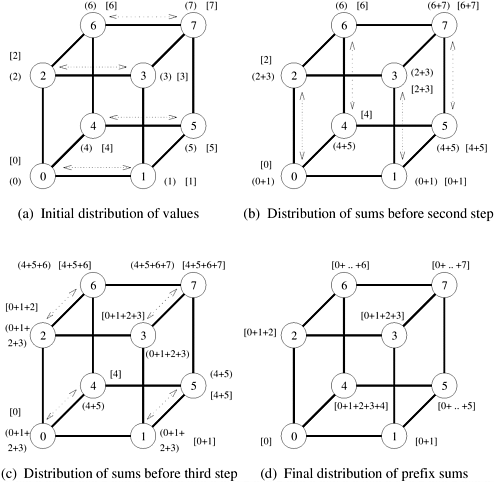
\includegraphics[width=1\textwidth]{hypercube.png}
    \caption{This figure shows the calculation of prefix sums with minimal communication phases. The figure is take from \cite[chap 4.3]{grama2003}}
    \label{fig:hypercube}
\end{figure}

Below follows pseudo code for parallel hypercube prefix sum (from \cite{grama2003}):

\begin{verbatim}
procedure PREFIX_SUMS_HCUBE(my_id, my number, d, result) 
   begin 
      result := my_number; 
      msg := result; 
      for i := 0 to d - 1 do 
          partner := my_id XOR 2i; 
          send msg to partner; 
          receive number from partner; 
          msg := msg + number; 
          if (partner < my_id) then result := result + number; 
      endfor; 
   end PREFIX_SUMS_HCUBE
\end{verbatim}



\subsection*{MPI Program using MPI\_Scan}
A minimal working example using MPI\_Scan.
\begin{verbatim}
#include <stdio.h>
#include <stdlib.h>
#include <mpi.h>
#include <time.h>

int main(void){

  int my_rank, comm_sz;
  int* initial_vector;
  int* prefix_sums;

  MPI_Init(NULL, NULL);
  MPI_Comm_rank(MPI_COMM_WORLD, &my_rank);
  MPI_Comm_size(MPI_COMM_WORLD, &comm_sz);
  srand(time(NULL));


  initial_vector = (int *) malloc(10*sizeof(int));
  prefix_sums = (int *) calloc(10, sizeof(int));

  for(int i = 0; i < 10;i++){
    initial_vector[i] = rand() % 1000;
  }

  MPI_Scan(initial_vector, prefix_sums, 10,MPI_INT, MPI_SUM, MPI_COMM_WORLD);

  for(int i = 0; i< comm_sz;i++){
    if (i == my_rank){
      for(int j = 0;j < 10;j++){
        printf("%d ", prefix_sums[j]);
      }
    }
  }
  printf("\n");

  MPI_Finalize();
  return 0;
}
\end{verbatim}

\section{3.13 - Generalization of vector scaling and dot product}

Below follows an implementation of the `Vector Scaling and Dot Product' using `MPI\_Scatterv'/`MPI\_Gatherv'.

\begin{verbatim}
#include <stdio.h>
#include <mpi.h>
#include <string.h>
#include <stdlib.h>
#include <time.h>


int main(int argc, char *argv[]) {
  int my_rank, comm_sz;
  int n, local_n, local_dotp_sum = 0, scalar, result_dot;
  int* sendcounts;
  int* displs;
  int* local_vec1;
  int* local_vec2;
  int* vector1;
  int* vector2;

  /* Initializing */
  MPI_Init(NULL, NULL);
  MPI_Comm_rank(MPI_COMM_WORLD, &my_rank);
  MPI_Comm_size(MPI_COMM_WORLD, &comm_sz);
  srand(time(NULL));

  /* Obtaining Data */
  if(my_rank==0 && argc > 1){

    if(strcmp(argv[1], "r") == 0){
      printf("using random data, vector length = %d\n", 100*comm_sz);
      n = 100*comm_sz;
      vector1 = (int *) malloc(100*comm_sz * sizeof(int));
      vector2 = (int *) malloc(100*comm_sz * sizeof(int));

      for(int i = 0; i < n;i++){
	vector1[i] = rand() % 1000;
	vector2[i] = rand() % 1000;
      }
      scalar = rand() % 1000;
    }
    
  } else if (my_rank==0){
     
    printf("enter vector length\n");
    scanf("%d", &n);
    printf("enter integer vector 1\n");

    vector1 = (int *) malloc(n * sizeof(int));
    vector2 = (int *) malloc(n * sizeof(int));

    for(int i = 0; i < n; i++){
      scanf("%d", &vector1[i]);
    }

    printf("enter integer vector 2\n");

    for(int i = 0; i < n; i++){
      scanf("%d", &vector2[i]);
    }

    printf("enter integer scalar\n");
    scanf("%d", &scalar);
  }

  /* Distribute Data */
  MPI_Bcast(&n, 1, MPI_INT, 0, MPI_COMM_WORLD);

  /* Fixing sendcounts for general n */
  sendcounts = (int *) malloc(comm_sz * sizeof(int));
  displs = (int *) calloc(comm_sz,  sizeof(int));

  for(int i = 0; i < comm_sz;i++){
    if(n % comm_sz > i){
      sendcounts[i] = (n/comm_sz) + 1;
    } else {
      sendcounts[i] = (n/comm_sz);
    }

  }

  for(int i = 1; i <comm_sz; i++){
    displs[i] = displs[i-1]+sendcounts[i];   
  }

 
  local_n = sendcounts[my_rank];

  local_vec1 = (int*) malloc(local_n * sizeof(int));
  local_vec2 = (int*) malloc(local_n * sizeof(int));
  
  MPI_Bcast(&scalar, 1, MPI_INT, 0, MPI_COMM_WORLD);
  MPI_Scatterv(vector1, sendcounts, displs, MPI_INT, local_vec1, sendcounts[my_rank], MPI_INT, 0, MPI_COMM_WORLD);
  MPI_Scatterv(vector2, sendcounts, displs, MPI_INT, local_vec2, sendcounts[my_rank], MPI_INT, 0, MPI_COMM_WORLD);

  
  /* Calculations */
  /* Calculate Dot Product */
  for(int i = 0;  i< local_n; i++){
    local_vec2[i]*=local_vec1[i];
  }

  /* Calculate vector-scalar product */
  for(int i = 0; i< local_n; i++){
    local_vec1[i]*=scalar;
  }

  /* Summing for dot product */
  for(int i = 0; i < local_n; i++){
    local_dotp_sum += local_vec2[i];    
  } 
 
  /* Collect Data */
  MPI_Gatherv(local_vec1, sendcounts[my_rank], MPI_INT, vector1, sendcounts, displs, MPI_INT, 0, MPI_COMM_WORLD); 
  MPI_Reduce(&local_dotp_sum, &result_dot, 1, MPI_INT, MPI_SUM, 0, MPI_COMM_WORLD);

  /* Results */
  if(my_rank == 0){
    printf("dot product = %d\n", result_dot);

    printf("vector-scalar product = ");
    for(int i = 0; i < n;i++){
      printf("%d ", vector1[i]);
    }
    printf("\n");
  }

  /* Clean up */
  if(my_rank==0){
    free(vector1);
    free(vector2);
  }
  
  free(local_vec1);
  free(local_vec2);

  MPI_Finalize();

  return 0;
} 

\end{verbatim}



\section{3.16 - Diagram for a butterfly implementation of allgather}

\begin{figure}
  \centering
    
\includegraphics[width=1\textwidth]{allgather.png}
    \caption{This figure shows a butterfly allgather implementation for 8 cores and a vector of length 16.}
    \label{fig:allgather}
\end{figure}



\section{3.18 - Derived data types}
takes a while to solve
requires programming

\section{3.20 - Pack and unpack}
requires programming


\section{3.21 - Matrix-vector multiplication}
takes a while to solve
requires programming
requires testing

\section{3.22 - Timing the trapezoidal rule}
takes a while to solve
Requires programming
requires testing

\section{3.27 - Speedup and efficienciy of odd-even sort}


\addcontentsline{toc}{section}{\refname}
\bibliography{references}

\end{document}
